\section{Test Case Generation through Deep Learning}

Figure~\ref{fig:deeptune} shows the test case generation process. Our compiler test case generation approach consists of two parts: first, extending the state-of-the-art in deep learning program synthesis; the second, a general application of established differential testing methodologies for running code samples.


\subsection{OpenCL Kernel Synthesis}

We extend prior work on synthetic program generation using LSTM networks~\cite{Cummins2017a}. An initial seed corpus of 10k OpenCL kernels is mined from GitHub, using an oracle compiler (LLVM 3.9) to reject files that are not well-formed or do not contain instructions. The corpus is preprocessed: a uniform code style is enforced to ensure consitent use of braces, whitespace, identifier names, etc. The prepocessed corpus is encoded using a hybrid token/character-level encoding~\cite{Cummins2017b}. 

LSTM networks model the vocabulary distribution over the encoded corpus. We use a two layer LSTM network of 512 nodes each, trained for 50 epochs using an initial learning rate of 0.002 and decaying by a factor of a half every 5 epochs.

The trained network is sampled to generate new programs. The model is seeded with the start of a kernel (\texttt{\_\_kernel void}), and sampled token-by-token until the brackets match, or until a pre-determined maximum number of tokens has been reached.


\begin{figure}
  \centering
  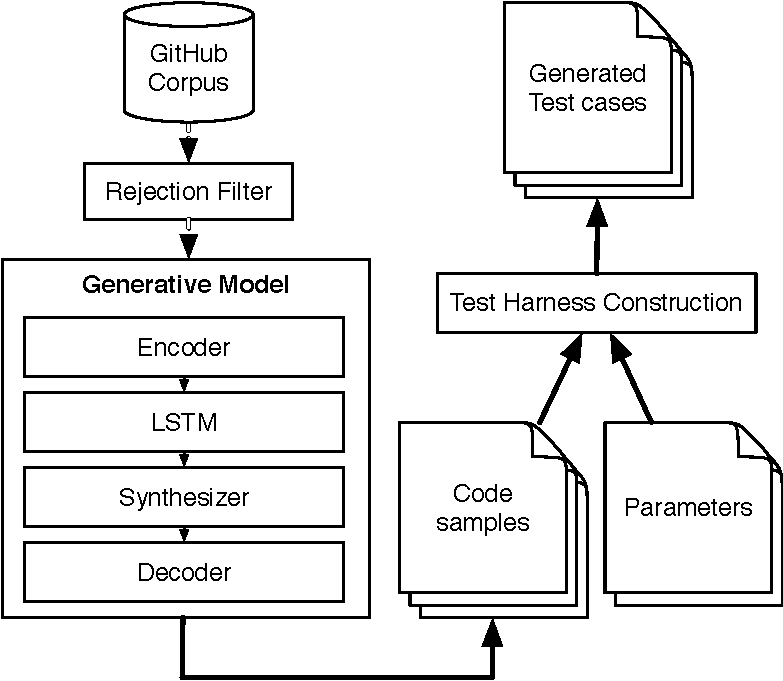
\includegraphics[width=.80\columnwidth]{img/clgen} %
  % \vspace{-2em}%
  \caption{%
    Test-case generation. An corpus of programs from GitHub is used to seed a generative model for program codes, whose outputs are parameterized to construct test cases.%
  }%
  \label{fig:deeptune}
\end{figure}


\subsection{Test Harness Construction}

OpenCL compute kernels requires host code (\emph{test harness}) to compile the kernel and feed with it inputs, then to print the outputs.

At first, we used the test harness of CLSmith. CLSmith kernels accept no inputs, and each thread computes the same value which is stored in a \texttt{unsigned long} buffer. The fixed function prototype means that they have a single re-usable test harness which compiles the kernel, runs it, and prints the results. We found this fixed harness to be too inflexible for our needs. This prototype is not a common OpenCL use case (only 5.6\% of GitHub kernels accept a single argument, of which 3.4\% are \texttt{ulong}, 0.2\% of the total).
% $ grep -E '^__global (.*)\* A$' github-arguments.txt | wc -l     -> 294
% $ grep '^__global ulong\* A$' ~/src/project_b/difftest/github-arguments.txt | wc -l     -> 10
To test a more expressive range of kernels, we created \emph{cldrive}, a tool to generate test harnesses for arbitrary OpenCL kernels.

We use cldrive to generate a unique test harness for every OpenCL sample we generate; the test harness has the OpenCL kernel embedded within it. If the sample is well-formed (i.e. it can be parsed), the test harness creates a \emph{payload} of buffers and values to match the function signature; else if the sample is ill-formed we generate a compile-only stub. 

Cldrive is the only language-specific component of our software stack. We support a limited subset of data types for kernel inputs: no structs, no irregular data types (this is just an implementation detail, and can be addressed with more dev time). \cc{cldrive is XX lines of code}.
